\chapter[Lab study of my population]{Extensive lab study reveals exciting results in my study system}
\label{chap:labstudy}

\begin{abstract}
  Here is the chapter abstract.
\end{abstract}

\section{Introduction}

Here is the introduction.

\begin{figure}[p]
  \centering
  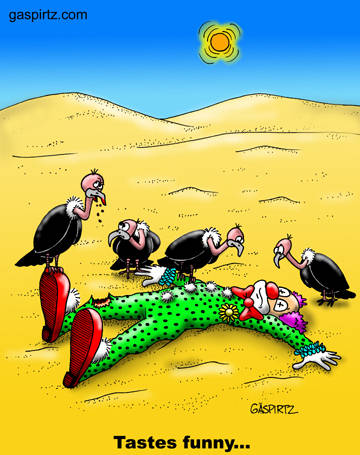
\includegraphics[width=.95\textwidth]{missingdata/figures/Tastes_funny.jpg}%Note that this is the path for the folder
  %for chapter 2 that has the Tastes_funny.jpg file within it.
  \caption[Vultures]{Long explanation of the figure}
  \label{fig:vultures}
\end{figure}

\section{We all love a few equations}
We like to put in some equations for a bit of fun.
where $\lambda_i$ is the speciation rate in state $i$, $\mu_i$ is the
extinction rate in state $i$, and $q_{ij}$ is the rate of transition
from state $i$ to $j$ forward in time.

\section{Results}
We briefly present the results of our lab work and equations


\section{Discussion}

Here is the discussion
